
\chapter{Tehtävä 4 \label{chap:Teht=0000E4v=0000E4-4}}

Tehtävänä oli luoda geneerinen Hajautustaulu ja Linkitetty lista ja kuvata niiden toimintaa visuaalisesti 
OOMKitillä. 

\section{Hajautustaulu}

\label{Hajautustaulu}

Hajautustaulu on luotu olio taulukko ArrayListina.(java ei anna tehdä geneerisiä taulukoita). 
Jossa samanlaiset oliot tallennetaan samalle sarakeelle. 
\label{Hajautustaulu}
\begin{javacode}
import java.util.ArrayList;


public class Hajautustaulu<E> {
	ArrayList<Object[]> list = new ArrayList<Object[]>();
	
	public Hajautustaulu() {
		 
	}
	public boolean lisää(E arvo) {
		for (Object[] taulu : list) {
			if(taulu[0].equals(arvo)) {
				for(int i=1;i<taulu.length;i++) {
					if(taulu[i] == null) {
						taulu[i]=arvo;
						return true;
					}else {
						return false;
					}
				}
			}
		}
		Object[] t = {arvo,null,null};
		list.add(t);
		return true;
		
	}
	public boolean poista(E arvo) {
		for(Object[] taulu : list) {
			if(taulu[0].equals(arvo)) {
				for(int i=0;i<taulu.length;i++) {
					if(taulu[i+1] == null) {
						taulu[i]=null;
						if(i == 0) {
							list.remove(taulu);
						}
						return true;
					}
				}
			}
		}
		return false;
	}
	
	
}

\end{javacode}

Ja visuaalisen kuvauksen tein omana metodinaan joka piirtää taulukon SimpleCanvasiin. 

\begin{javacode}
 public void piirräHajautustaulu(GraphicsContext gc,Hajautustaulu<CoreColor> h) {
            	for (int i=0;i<h.list.size();i++) {
           			for(int j=0;j<h.list.get(i).length;j++) {
           				if(h.list.get(i)[j] != null) {
           					gc.setFill(((CoreColor)(h.list.get(i)[j]))
                                                                  .toFXColor());
            				gc.fillRect(i*60+100,j*60+100,60,60);
           				}else {
        					gc.setFill(Color.WHITE);
        					gc.fillRect(i*60+100,j*60+100, 60, 60);
        				}
        				gc.strokeRect(i*60+100,j*60+100,60,60);
        			}
        		}
           	}

\end{javacode}

Kuva miltä hajautustaulu näyttäisi.



\begin{figure}
\centering 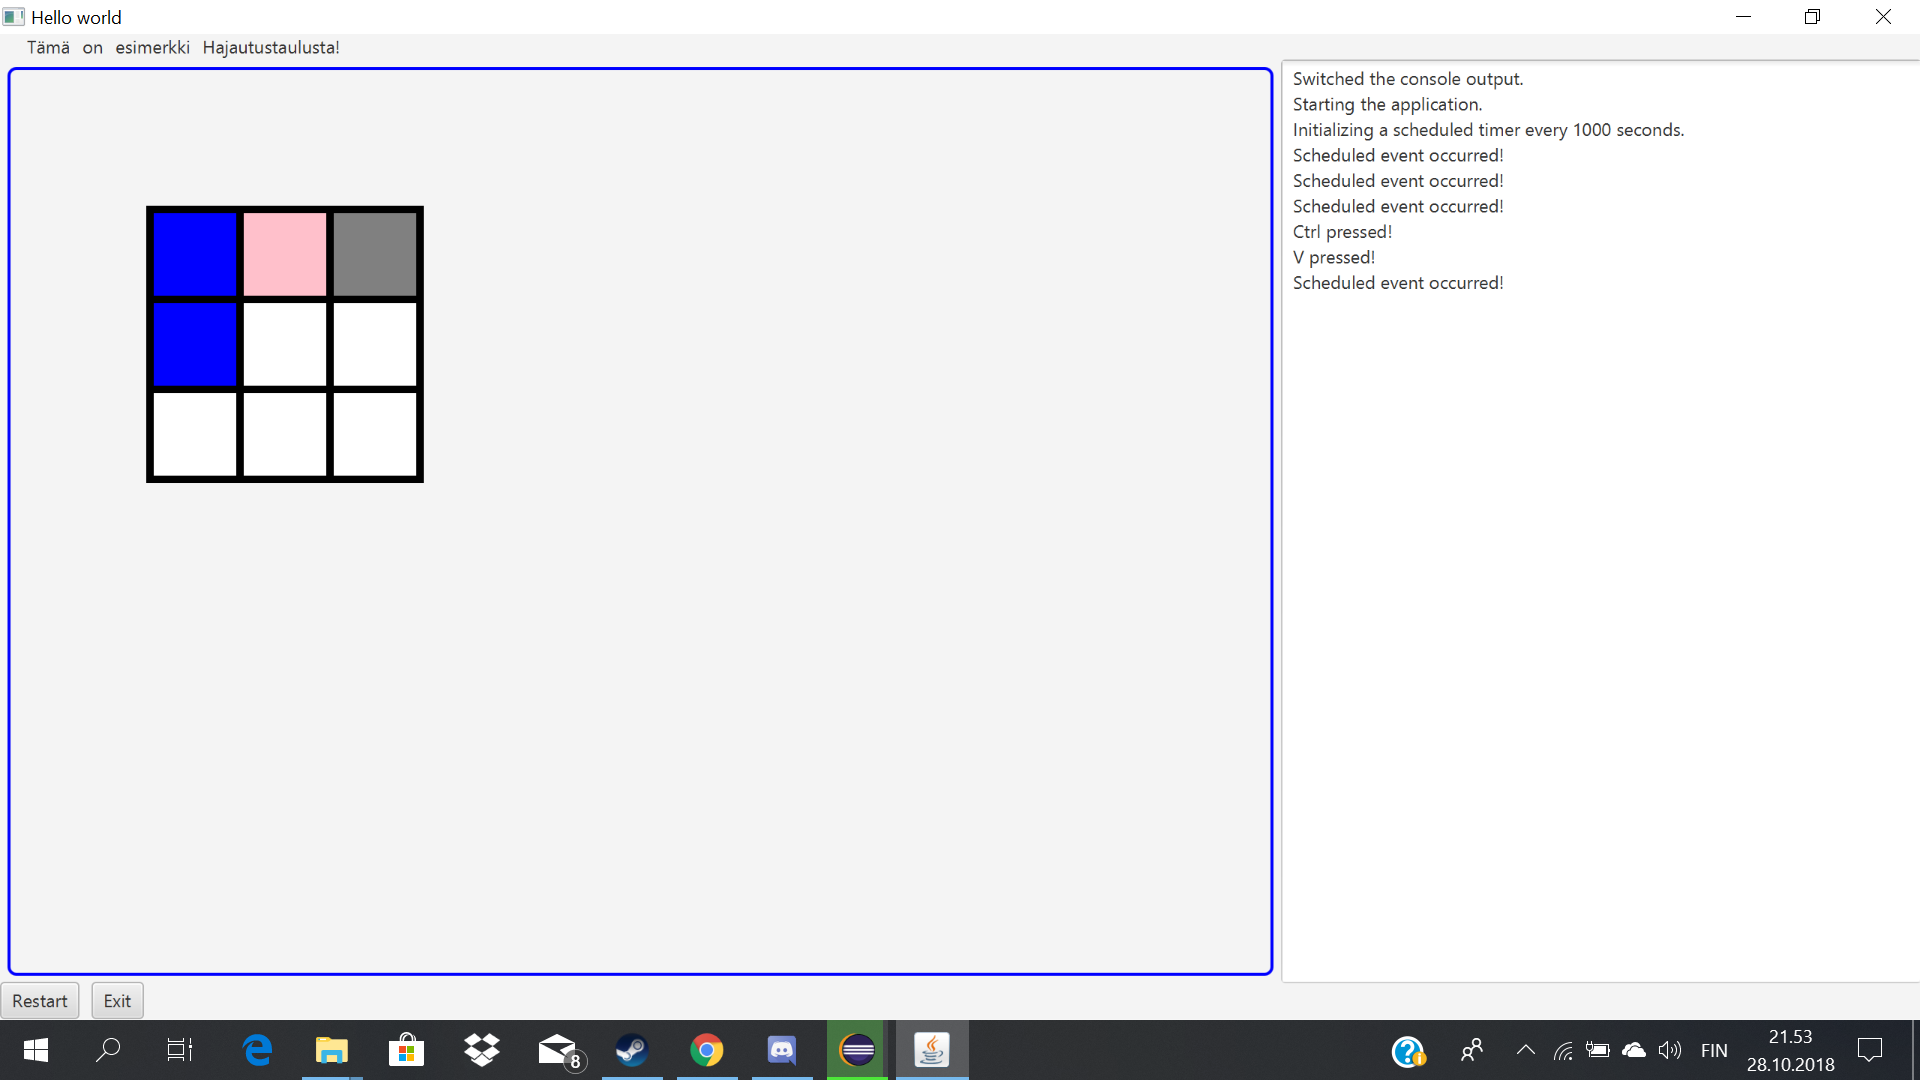
\includegraphics[width=0.5\textwidth]{kuvat/Hajautustaulu}
\label{Hajautustaulu} 
\end{figure}



\section{Linkitetty lista}

\label{Linkitetty lista}
 Toinen tehtävän osa oli linkitetty lista, joka oli mielästäni paljon helpompi toteutaa. Tein perus yksisuuntaisen linkitetyn listan 
 jossa alkio tietää oman arvonsa ja mitä tulee sen jälkeen.
 \begin{javacode}
 
 public class LinkitettyLista<E> {
	E arvo;
	LinkitettyLista<E> seuraava;
	
	public LinkitettyLista(E arvo) {
		this.arvo = arvo;
		seuraava = null;
	}
	
	public void lisää(E arvo) {
		E tempt = this.arvo;
			if(seuraava != null) {
				tempt = seuraava.arvo;
				seuraava.lisää(arvo);			}
			else {
				seuraava = new LinkitettyLista<E>(arvo);
		}
	}
		
				
	
	public boolean poista(E arvo) {
		LinkitettyLista<E> edellinen = null;
		LinkitettyLista<E> temp = this;
		do {
			if(temp.arvo.equals(arvo)) {
				if(edellinen != null) {
					if(temp.seuraava != null) {
						edellinen.seuraava = temp.seuraava;
						return true;
					}else {
						edellinen.seuraava = null;
						return true;
					}
				}
			}
			edellinen = temp;
			temp = edellinen.seuraava;
		}
		while(temp.seuraava != null);
		return false;
	}
	public void tulosta() {
		LinkitettyLista solmu = this;
		System.out.println(solmu.arvo.toString());
		
		while(solmu.seuraava != null) {
			solmu = solmu.seuraava;
			System.out.println(solmu.arvo.toString());
		}
	}
}
    
\end{javacode}

Linkitetylle listalle on myös sen oma piirtämismetodi. Linkitetty lista piirretään ainasamaan kohtaan ja sen lopuun tulee 
musta neliö. 

\begin{javacode}

public void piirräLinkitettyLista(GraphicsContext gc,LinkitettyLista<CoreColor> lista) {
            	LinkitettyLista solmu = lista;
            	int x = 100;
                int y = 100;
        		//System.out.println(solmu.arvo.toString());
            	gc.setFill(((CoreColor)(solmu.arvo)).toFXColor());
            	gc.fillRect(x, y, 60, 60);
            	gc.strokeRect(x,y,60,60);
            	x = x+60;
        		
        		while(solmu.seuraava != null) {
        			solmu = solmu.seuraava;
        			gc.setFill(((CoreColor)(solmu.arvo)).toFXColor());
                	gc.fillRect(x, y, 60, 60);
                	gc.strokeRect(x,y,60,60);
                	x = x+60;
        		}
        		gc.setFill(Color.BLACK);
            	gc.fillRect(x, y, 60, 60);
            	gc.strokeRect(x,y,60,60);
            	
            }
	    
	    
\end{javacode}
Kuva miltä linkitetty lista näyttää OOMKitillä.


\begin{figure}
\centering 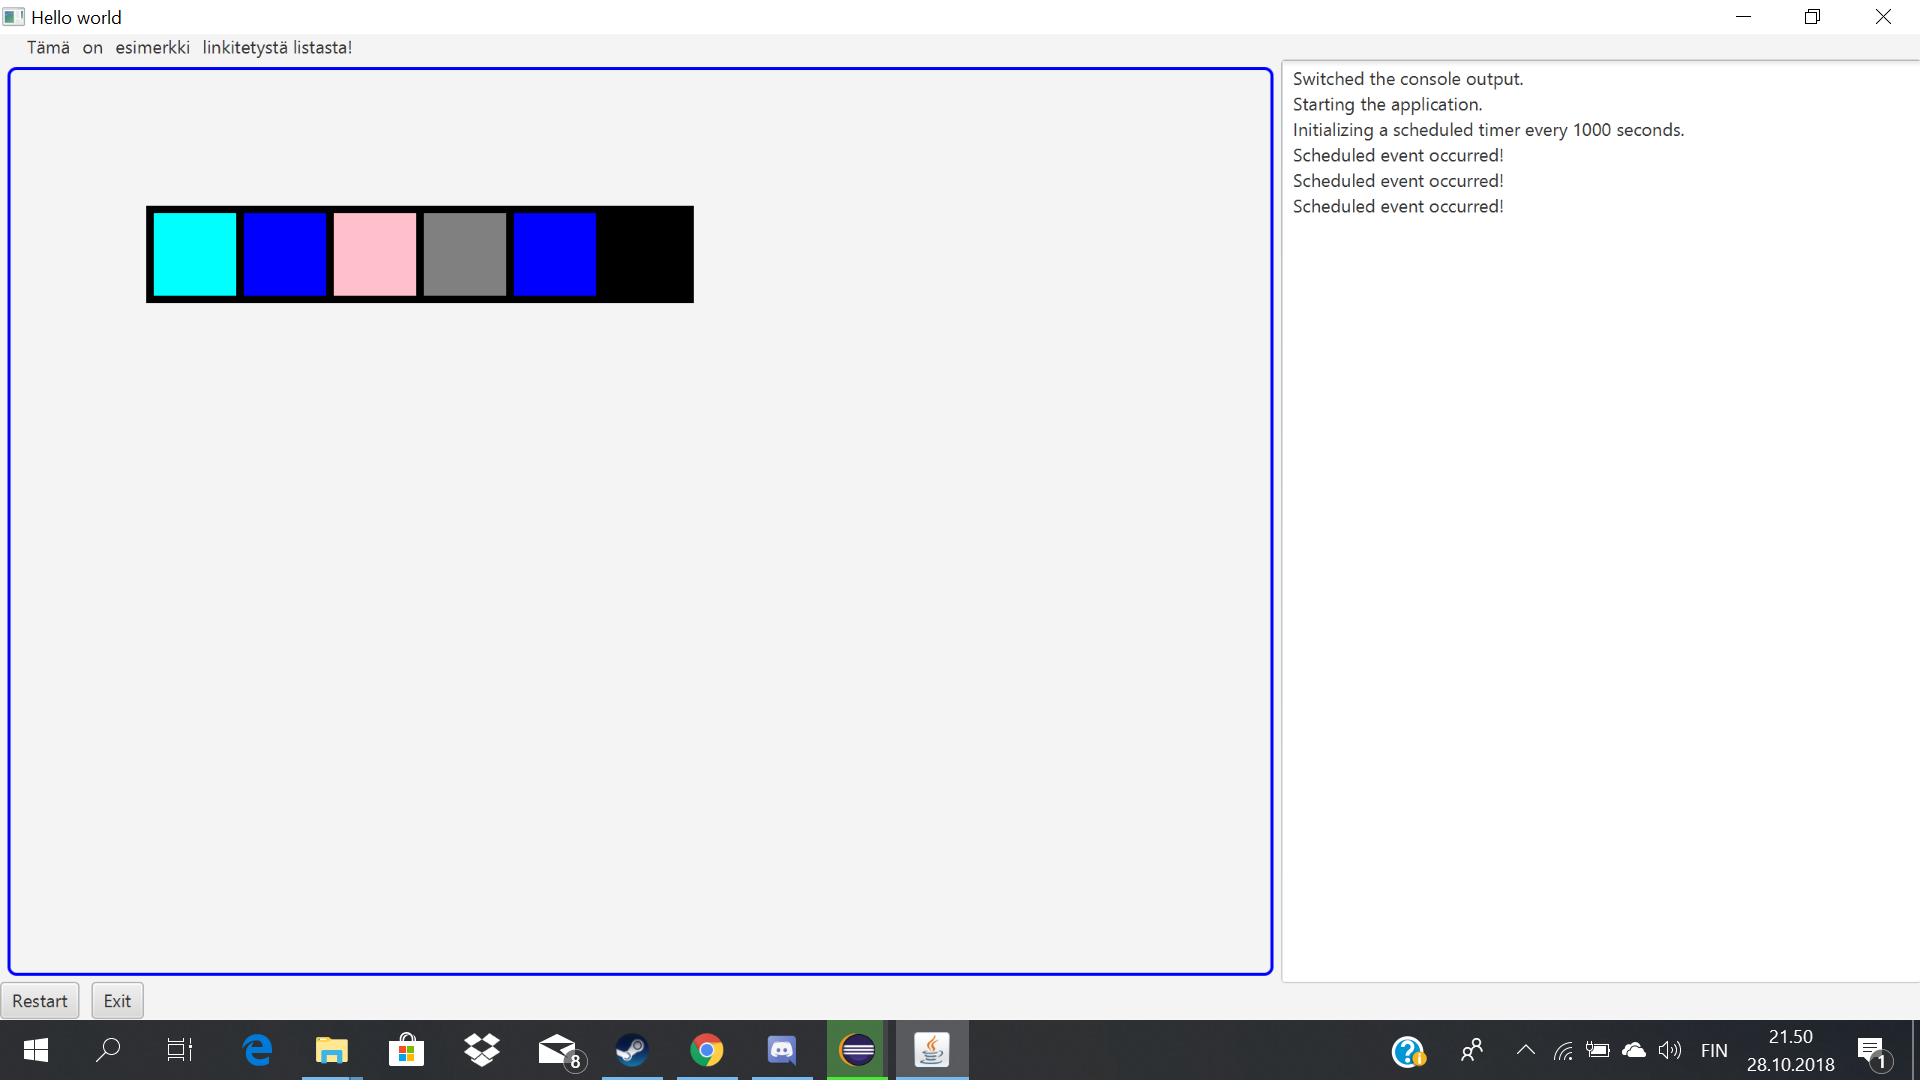
\includegraphics[width=0.5\textwidth]{kuvat/LinkitettyLista}
\label{LinkitettyLista} 
\end{figure}





Tekijänä Janina Kuosmanen (516580)

\label{endofpages}
